\documentclass{article}
\usepackage[utf8]{inputenc}
\usepackage{natbib}
\usepackage{graphicx}
\usepackage{hyperref}
\usepackage{enumerate}
\newcounter{saveenumi}
\newcommand{\seti}{\setcounter{saveenumi}{\value{enumi}}} %untuk setting melanjutkan penomoran
\newcommand{\conti}{\setcounter{enumi}{\value{saveenumi}}} %untuk setting melanjutkan penomoran
\usepackage{lipsum}
\title{Laporan Harian Proyek 1}
\author{Burhanudin Zuhri}
\date{April 2020}
\begin{document}

\maketitle
	\begin{center}
		
\includegraphics[width=8cm,height=8cm]{logo.png}
	\end{center}
	\vspace{0.5 cm}
	
	\begin{center}
		Burhanudin Zuhri \\
		1194008 \\
		1A D4 TI \linebreak
		\newline
		\newline
		\newline
		\linebreak
		\newline
		\newline
		PROGRAM STUDI D4 TEKNIK INFORMATIKA \\
		POLITEKNIK POS INDONESIA\\
		2019/2020\\
	\end{center}

\section{Tanggal 26 Maret 2020:}

Pada tanggal ini kami bergabung dengan grup bimbingan Mr. Awangga. Kami mendapat tugas pertama kami untuk menginstall navicat dan terkoneksi dengan database MySQL. Besoknya kami diberi tugas untuk mengisi tabel notfound\_message dan error\_message dengan persetujuan setiap kelompok memilih salah satu tabel tersebut. Serta setiap orang dari dari masing-masing kelompok harus mengisi 100 record. . Berikut merupakan langkah mendownload dan menginstal Navicat:
\newline
\begin{enumerate}
        \item Untuk menginstal \textbf{Navicat} kami mengunduh dahulu di internet di \textbf{website} resmi \textbf{Navicat}.
        \newline
        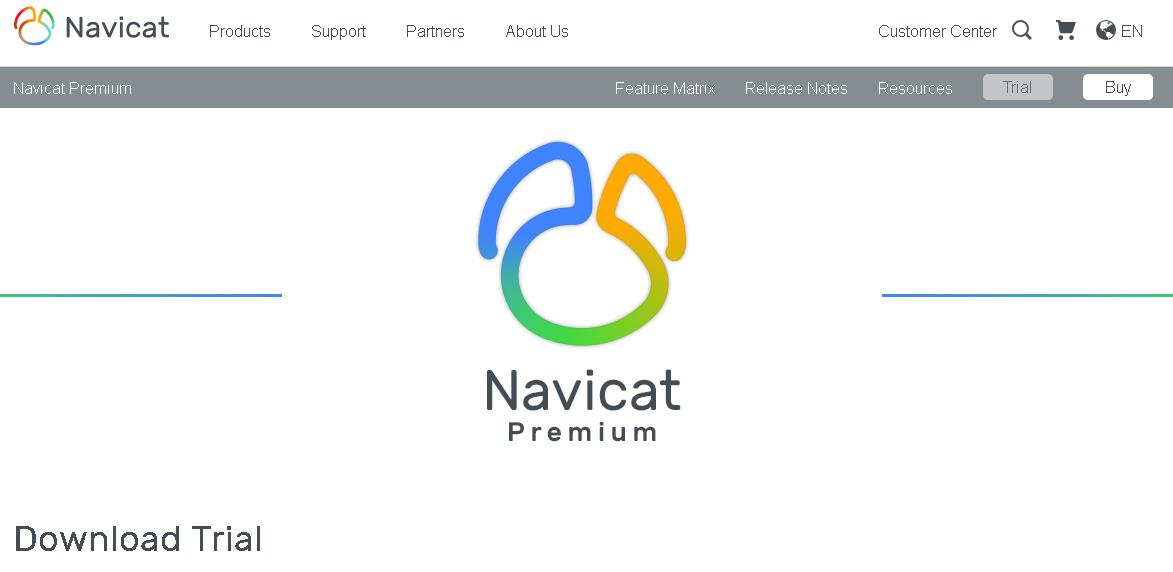
\includegraphics[scale=0.3]{26.1.jpg}
        \newline
        \item Kami memilih \textbf{Navicat} yang sesuai dengan spesifikasi laptop kami.
        \newline
        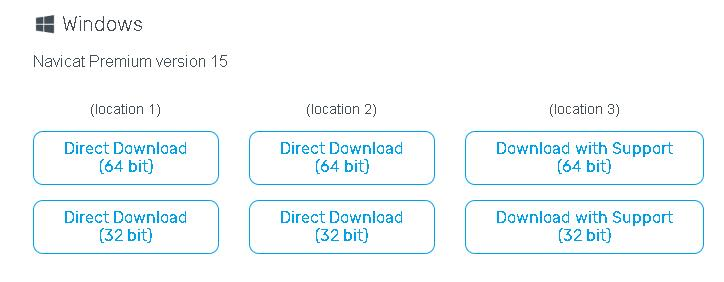
\includegraphics[scale=0.5]{26.2.jpg}
        \newline
        \item Setelah \textbf{Navicat} selesai diunduh, maka selanjutnya kami menginstal \textbf{Navicat}
        \newline
        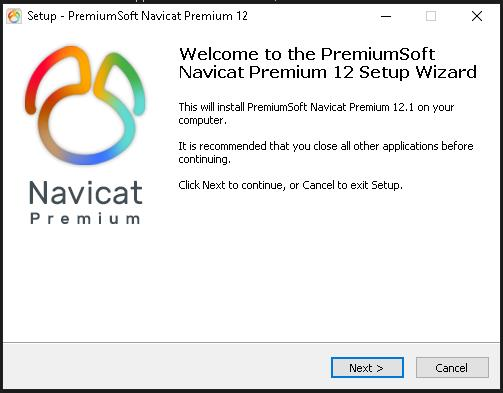
\includegraphics[scale=0.5]{26.3.jpg}
        \newline
        \item Jika \textbf{Navicat} sudah diinstal selanjutnya yaitu mengaktifkan \textbf{database} \textbf{MySQL} pada aplikasi \textbf{XAMPP} agar servis \textbf{MySQL} dapat berjalan
         \newline
        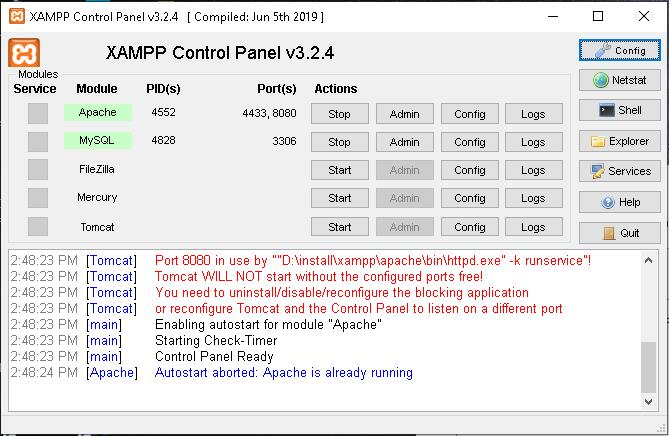
\includegraphics[scale=0.4]{26.4.jpg}
        \newline
        \item Mengerjakan tugas \textbf{error\_message} dan berhubung pada hari tersebut belum dapat menginputkan record pada database “bimbingan” maka kami menululiskan dahulu di \textbf{database} \textbf{MySQL}.
        \newline
        \newline
        a. Membuat koneksi  dengan cara menekan tombol icon Connection pada bagian kiri atas Navicat 
         \newline
        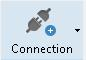
\includegraphics[scale=2]{26.5a.jpg}
        \newline
        b. Mengatur  host name,  port,  unsername, dan password MySQL
          \newline
        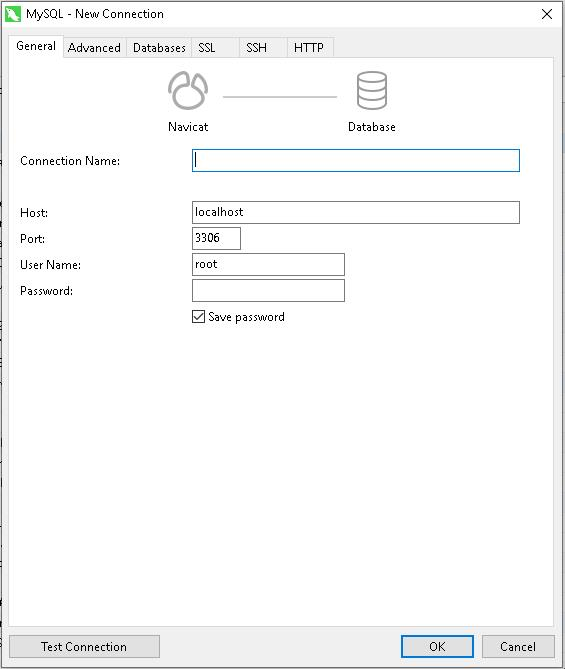
\includegraphics[scale=0.5]{26.5b.jpg}
        \newline
        c. Membuat databse baru dengan cara klik kanan padaMySQL dan pilih New Database lalu isi dengan nama bebas (disini saya menamainya dengan nama content\_chatbot)
        \newline
        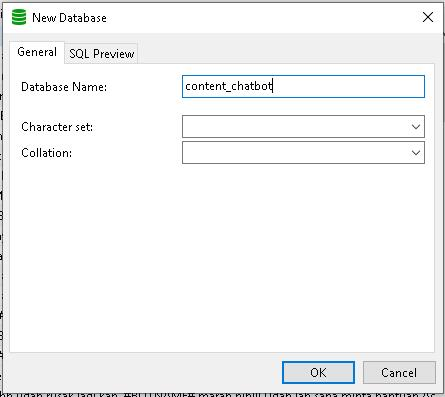
\includegraphics[scale=0.6]{26.5c.jpg}
        \newline
        d. Secara otomatis database yang  saya buat akan memiliki fitur untuk membuat table, view, backup, dan sebagainya. Disini saya memasukkan record saya untuk sementara.
        \newline
        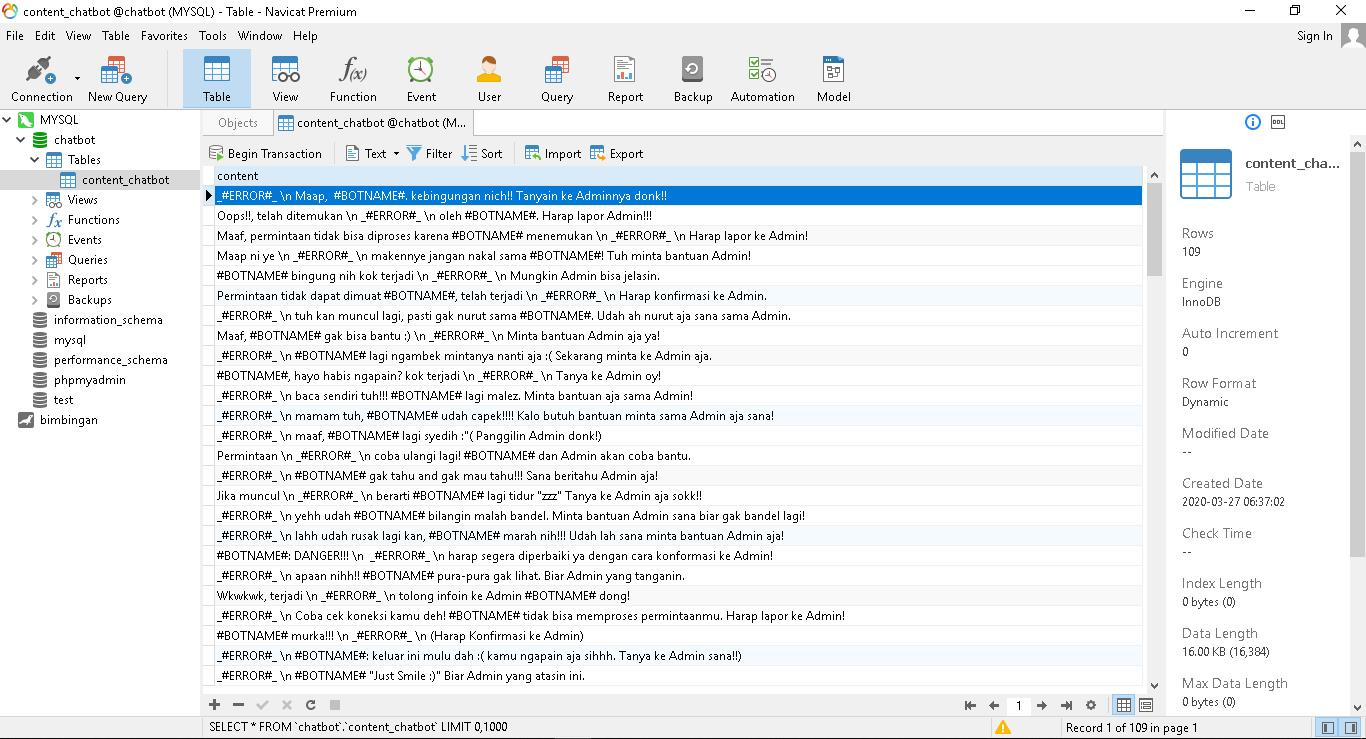
\includegraphics[scale=0.3]{26.5d.jpg}
        \newline
        \seti %harus diketik pada nomor terakhir
    \end{enumerate}


\section{Tanggal 28 Maret 2020:}
Kami telah menyelesaikan tugas pertama kami. Siang harinya, Bapak Rolly menjadwalkan pertemuan via google meet guna membahas cara menyambungkan navicat ke database mariadb. Setelah meeting dimulai, Bapak Rolly memberikan contoh bagaimana cara mengisi record. Sore harinya, Bapak Rolly meminta kami untuk merevisi kesalahan pada pekerjaan kami karena banyak dari kami yang mengerjakan pekerjaan kami yang belum sesuai dengan ketentuan Bapak Rolly. Berikut merupakan cara menghubungkan Navicat dengan database mariaDB
\newline
\newline
\begin{enumerate}
    \item Mengisi SSH dengan ketentuan
            \textbf{Name}  \textbf{=} \textbf{croot.ypbpi.or.id} \newline \textbf{Port} \textbf{=} 60606 \newline \textbf{User Name} \textbf{=} \textbf{if}
            \newline
            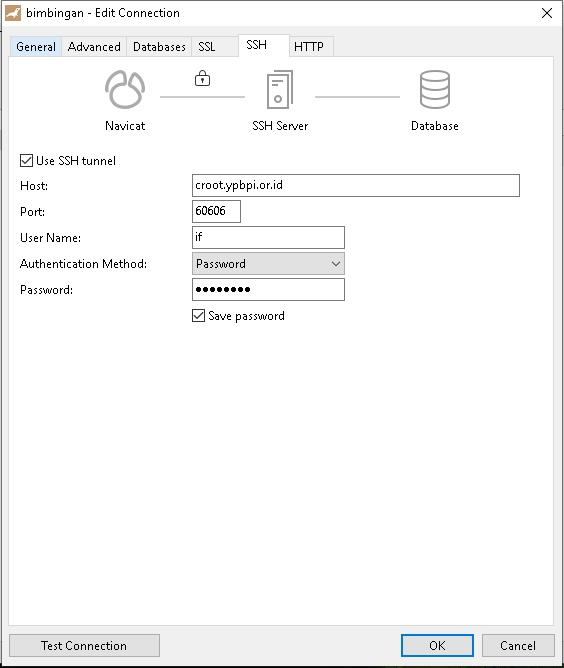
\includegraphics[scale=0.4]{28.1.jpg}
            \newline  
    \item Mengisi Database General dengan ketentuan 
            \textbf{Connection} \textbf{=} bimbingan (bebas) \newline \textbf{Host} \textbf{=} \textbf{192.168.1.223} \newline \textbf{Port} \textbf{=} 3306 \newline \textbf{User Name} \textbf{=} \textbf{if}
            \newline
            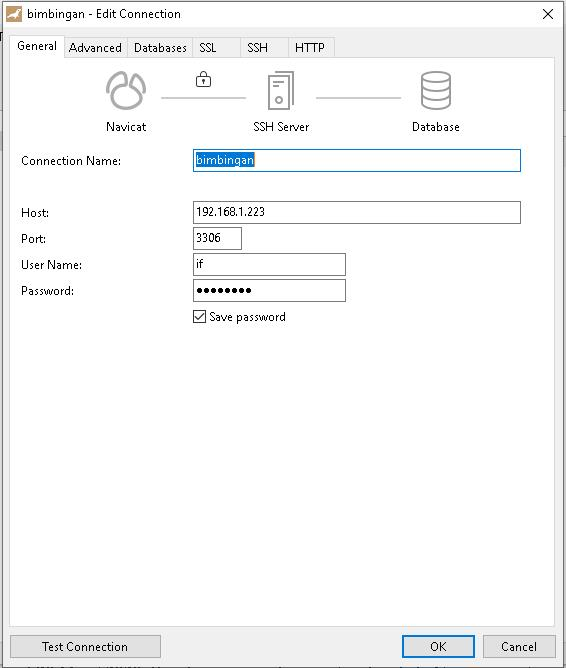
\includegraphics[scale=0.4]{28.2.jpg}
            \newline
    \item Setelah terhubung akan muncul “bimbingan” dengan 3 database yaitu information\_schema, test, dan wanda.
	        \newline
	        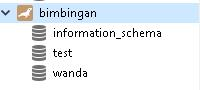
\includegraphics[scale=0.8]{28.3.jpg}
	        \newline
    \item Selanjutnya yaitu mengisikan record yang telah dibuat ke dalam database wanda dengan cara kilik 2x pada database wanda lalu akan muncul beberapa table error\_message, notfound\_message, opening\_message, dan waiting\_message.
		    \newline
		    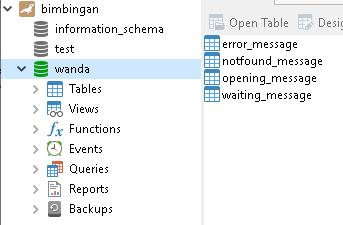
\includegraphics[scale=0.5]{28.5.jpg}
		    \newline
    \item Pilih error\_message lalu masukkan record di dalam content.
	        \newline
	        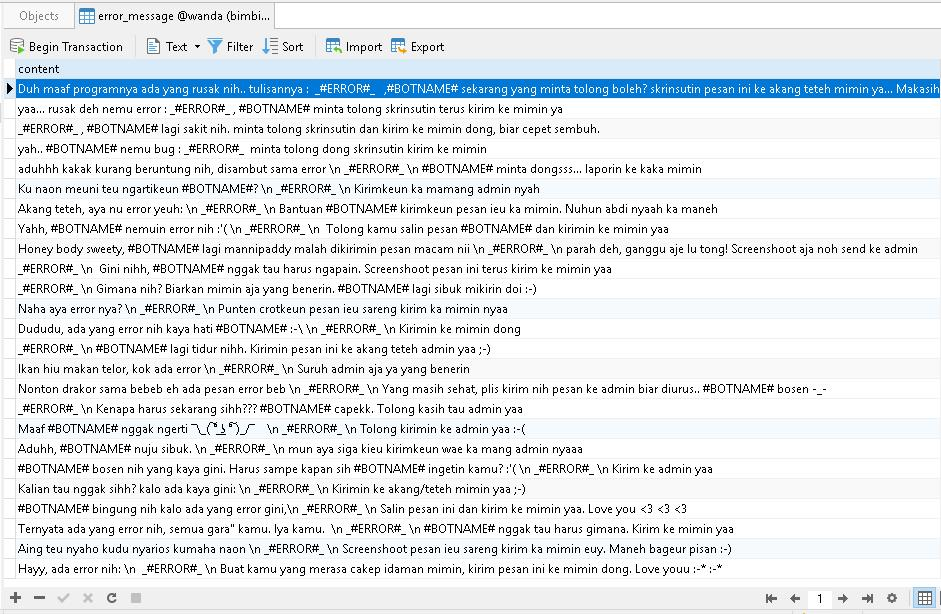
\includegraphics[scale=0.4]{28.4.jpg}
	        \newline
	\seti %harus diketik pada nomor terakhir
\end{enumerate}

\section{Tanggal 29 Maret 2020:}
Bapak menyarankan untuk memberi emoticon pada record kami. Kami menambahkan emoticon dan mengupdate record kami. Pada hari tersebut, Bapak Rolly merencanakan untuk melakukan pertemuan meeting lagi. Namun, karena ada beberapa hal, meeting tidak jadi dilaksanakan. Berikut merupakan beberapa contoh emoticon.
\newline
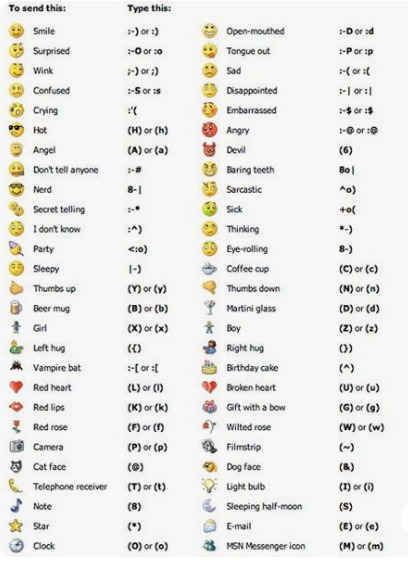
\includegraphics[scale=0.3]{29.1.jpg}
\newline

\includegraphics[scale=0.8]{29.2.jpg}
\newline


\section{Tanggal 30 Maret 2020:}
Bapak Rolly merencanakan untuk mengadakan meeting kembali. Namun, meeting tidak jadi dilaksanakan karena mungkin beberapa hal. 


\section{Tanggal 31 Maret 2020:}
Bapak Rolly memberikan tugas untuk mengisi opening\_message. Pada hari tersebut, bapak menginformasikan bahwa pada proyek 1 setiap orang memegang 1 modul. Setiap orang 1 modul ekisting dan 1 modul pengembangan. Setelah itu, Bapak Rolly memberi tugas untuk mengisi record ke dalam waiting\_message, yaitu antara lain kelas\_mulai, kelas\_selesai, dan jadwal\_kelas sebanyak 34 record per orangnya.
    \newline
    \newline
    \begin{enumerate}
        \item opening\_message
            \newline
            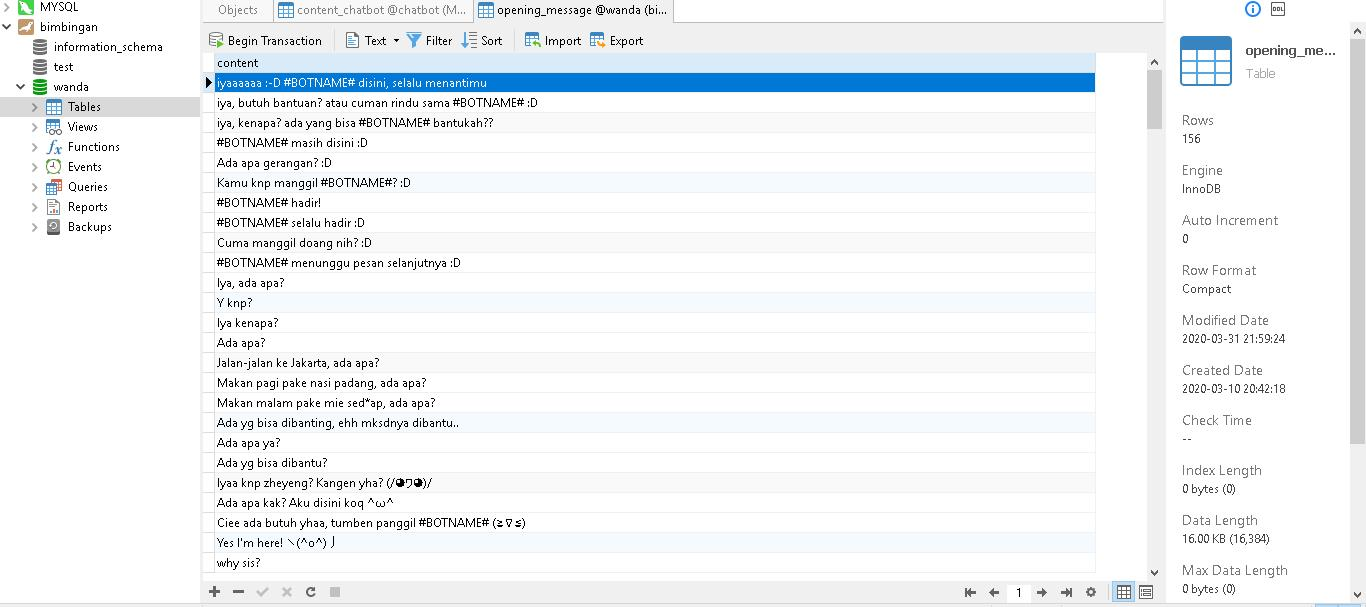
\includegraphics[scale=0.3]{31.1.jpg}
            \newline
        \item kelas\_mulai
            \newline
            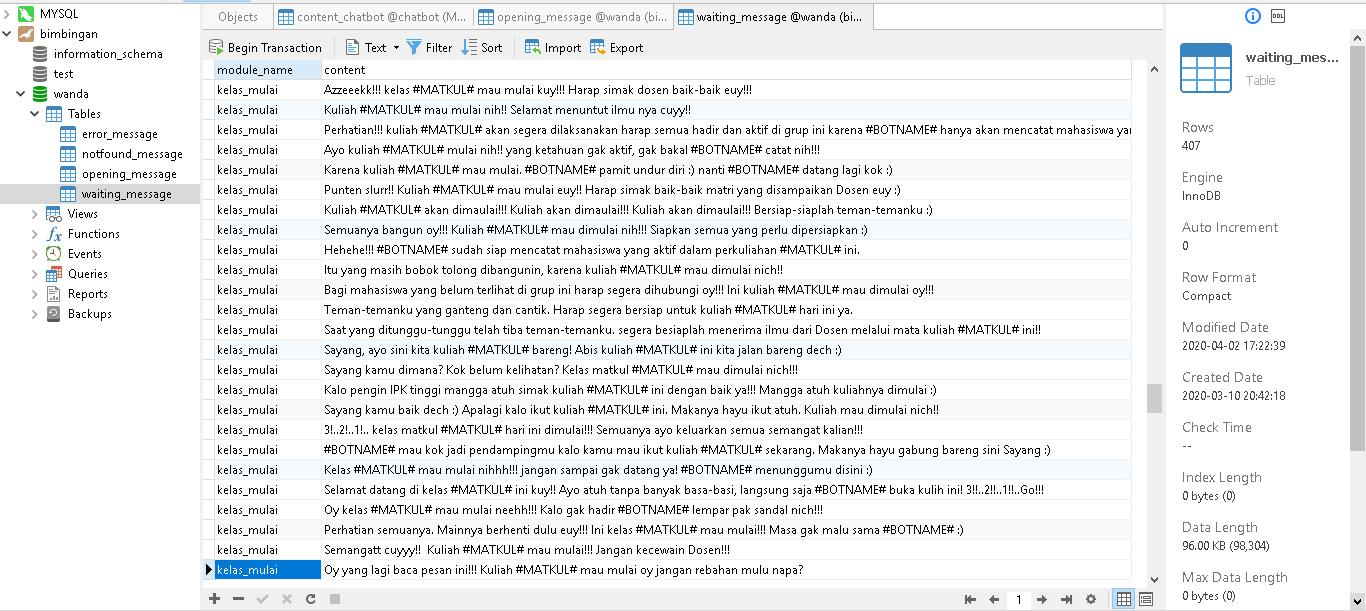
\includegraphics[scale=0.3]{31.2.jpg}
            \newline
        \item kelas\_selesai
            \newline
            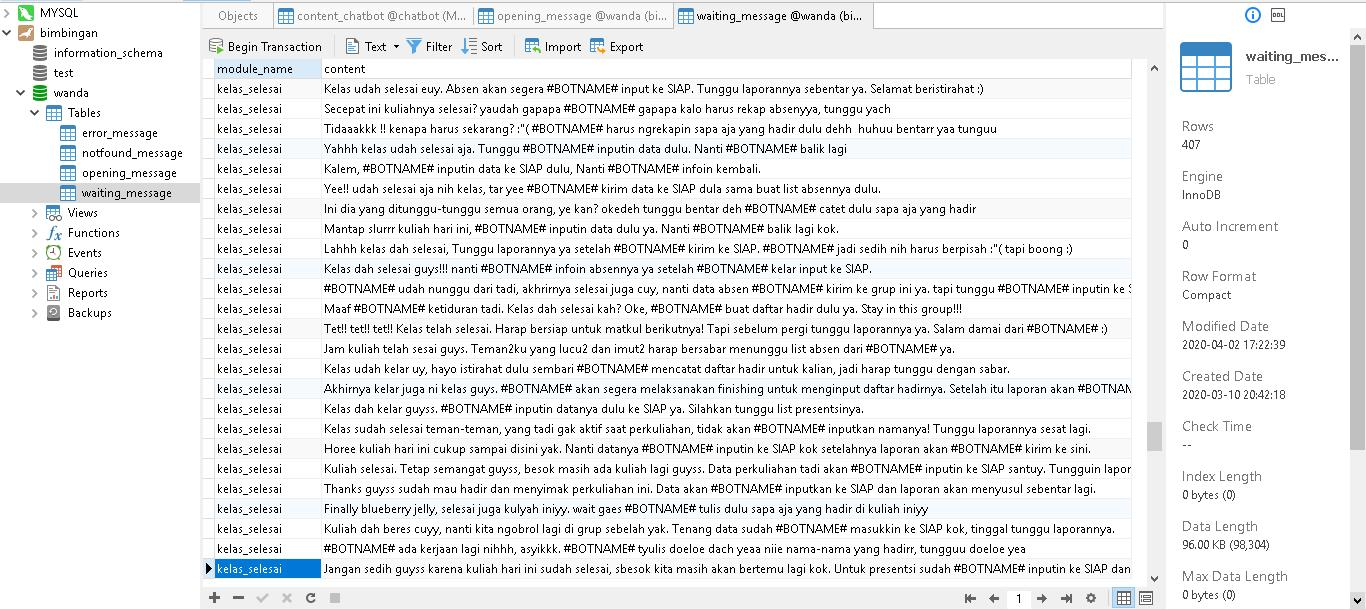
\includegraphics[scale=0.3]{31.3.jpg}
            \newline
        \item jadwal\_kelas
            \newline
            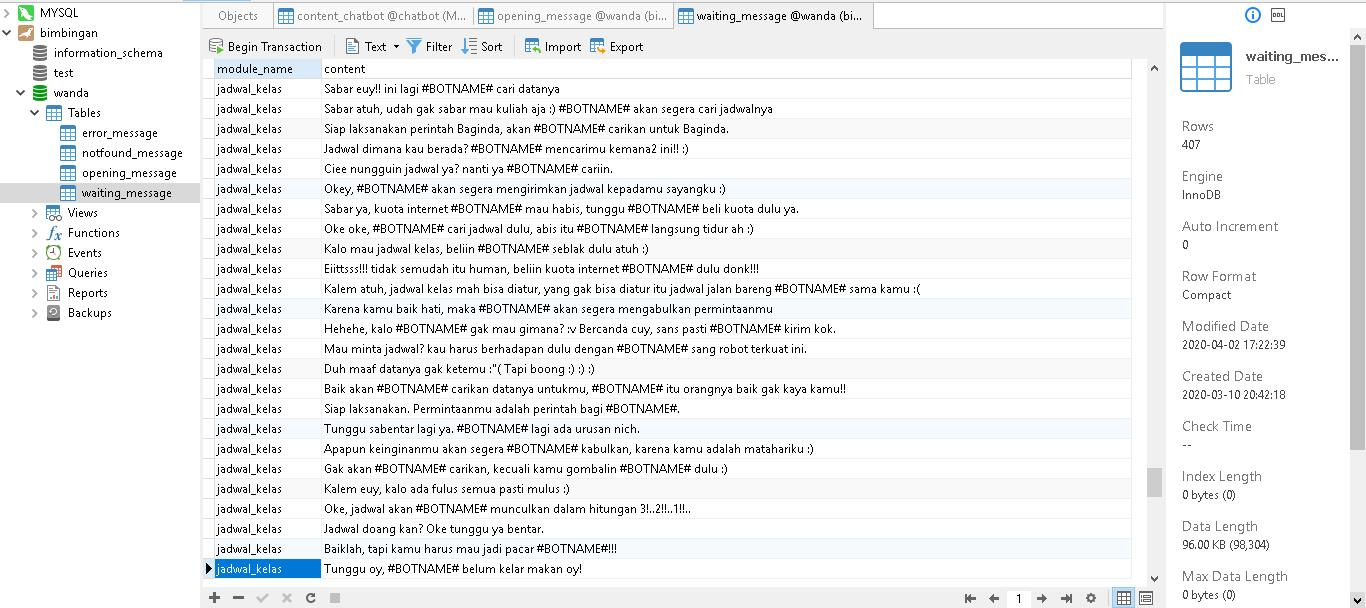
\includegraphics[scale=0.3]{31.4.jpg}
            \newline
          	\newline
            \seti %harus diketik pada nomor terakhir
        \end{enumerate}
     \begin{enumerate}
    	\item Penjelasan dari Tiap Table Database
    		\newline
        \item error\_message
            \newline
            \par Tabel ini berfungsi untuk memberitahukan kepada pengguna bahwa terjadi kesalahan pada sistem (error system). Table error \_message memiliki syarat yaitu harus memuat \_ERROR\_ dan BOTNAME. Sebagai tambahan bisa memasukkan “\\n” yang berfungsi sebagai baris baru (new line). Variable yang terdapat pada table yaitu \_ERROR\_ yang berfungsi menampilkan error yang terdapat pada aplikasi dan BOTNAME yang merupakan variable yang berfungsi sebagai nama robot.
            \newline
        \item notfound\_message
            \newline
            \par Table ini berfungsi untuk menjawab pesan yang tidak dapat diproses oleh robot. Jawaban yang diberikan oleh robot disesuaikan dengan bahasa sehari-hari manusia sehingga tidak terlihat seperti robot. Table ini hanya memiliki syarat harus memuat BOTNAME sebagai nama robotnya. Variable yang terdapat pada table yaitu BOTNAME Merupakan variable yang berfungsi sebagai nama robot.
            \newline
        \item opening\_message
            \newline
            \par Tabel  ini merupakan pesan respon  yang disampaikan robot karena telah menyebutkan nama robot. Variable yang terdapat pada table yaitu BOTNAME yang merupakan variable yang berfungsi sebagai nama robot.
            \newline
        \item waiting\_message
            \newline
            \par Tabel ini merupakan table yang berisi respon kepada pengguna untuk menunggu. Tabel ini memuat kelas\_mulai, kelas\_selesai, jadwal\_kelas. Variable yang terdapat pada table yaitu BOTNAME yang merupakan variable yang berfungsi sebagai nama robot.
            \newline
        	a. kelas\_mulai
            \newline
            \par Tabel ini merupakan pemberitahuan bahwa perkuliahan suatu mata kuliah akan segera dimulai. Tabel ini memiliki syarat yaitu harus memuat BOTNAME dan MATKUL. Variable yang terdapat pada table yaitu BOTNAME yang merupakan variable yang berfungsi sebagai nama robot dan MATKUL yang merupakan variable yang berfungsi sebagai mata kuliah yang akan dilaksanakan
            \newline
        	b. kelas\_selesai
            \newline
            \par Tabel ini merupakan pemberitahuan bahwa perkuliahan suatu mata kuliah sudah berakhir. Tabel ini memiliki syarat yaitu harus memberitahukan kepada pengguna bahwa robot akan menginputkan data ke SIAP dan mengirimkan laporannya ke grup tersebut. Variable yang terdapat pada table yaitu BOTNAME yang merupakan variable yang berfungsi sebagai nama robot.
            \newline
        	c. jadwal\_kelas
            \newline
            \par Tabel ini merupakan respon robot ketika pengguna meminta jadwal. robot akan mengirimkan jadwal ke grup tersebut ketika pengguna menggunakan kata kunci “jadwal kelas”. Variable yang terdapat pada table yaitu BOTNAME yang merupakan variable yang berfungsi sebagai nama robot.
            \newline
            \seti %harus diketik pada nomor terakhir
        \end{enumerate}

\section{Tanggal 1 April 2020:}
Bapak Rolly memberikan instruksi untuk belajar git dan selenium untuk website modul pengembangan. Dan akan dipandu oleh Kak Wahyu dan Kak Inal. Berdasarkan modul yang telah diberikan kami mengikuti langkah-langkah sebagai berikut:
    \newline
    \newline
     \begin{enumerate}
        \item Download dan install  Gitbash lalu membuat akun Github
	            \newline
	            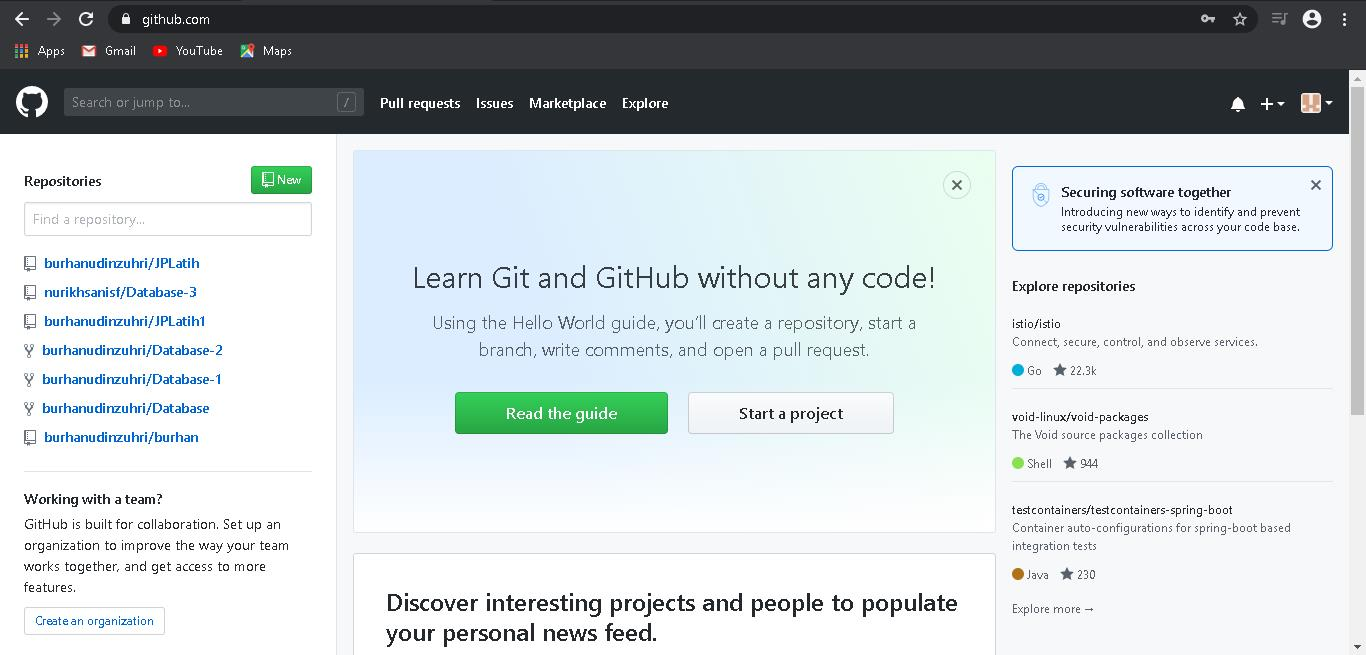
\includegraphics[scale=0.3]{32.1.jpg}
	            \newline
        \item Membuat akun GitLab, namun berhubung GitLab sudah terhubung dengan Github maka tidak perlu membuat akun, dan hanya sign in saja.
	        	\newline
       	\item Konfigurasi Key
                \newline
        	a. Buka Gitbash di home directory lalu ketik “cd” lalu Enter
                \newline
                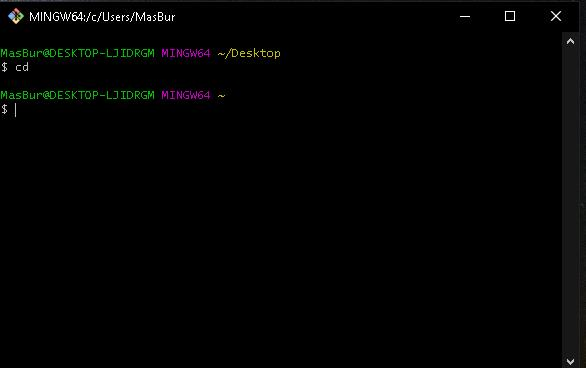
\includegraphics[scale=0.5]{32.3a.jpg}
                \newline
        	b. Ketik “ssh-keygen –t rsa –b 4096 –C “burhanudinzuhri25@gmail.com” (isi sesuai email anda)” dan  di perintah keygen ini, cukup dengan klik enter-enter saja.
                \newline
                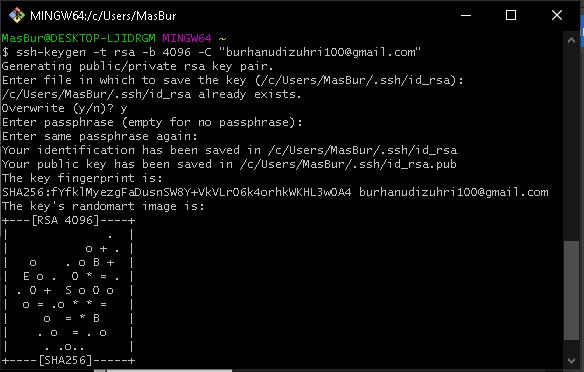
\includegraphics[scale=0.5]{32.3b.jpg}
                \newline
        	c. Masukkan perintah “cat . ssh/id\_rsa .pub” maka akan keluar hasilnya seperti ini
                \newline
                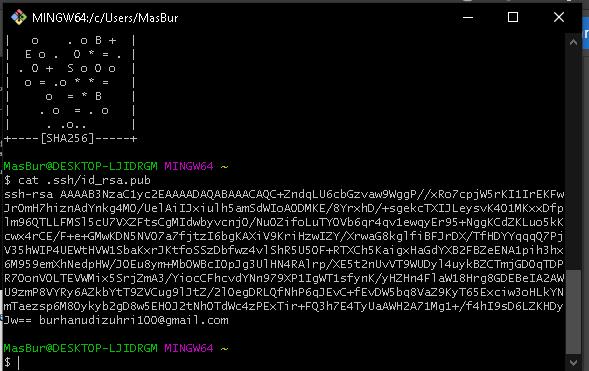
\includegraphics[scale=0.5]{32.3c.jpg}
                \newline
        	d. Selanjutnya masuk kea kun Github, klik Menu Setting, pilih menu SSH and GPG keys dan tambahkan New SSH key
                \newline
                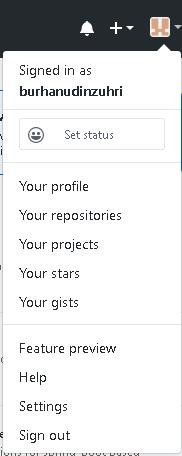
\includegraphics[scale=0.5]{32.3d.jpg}
                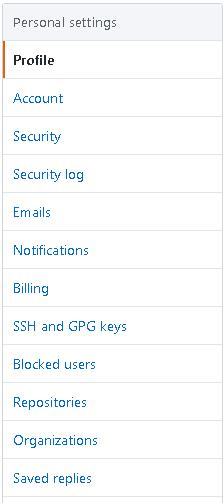
\includegraphics[scale=0.45]{32.3e.jpg}
                \newline
                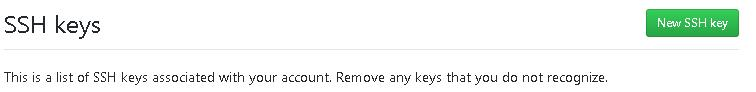
\includegraphics[scale=0.5]{32.3f.jpg}
                \newline
             \seti %harus diketik pada nomor terakhir
        \end{enumerate}
    \begin{enumerate}
    \item Penjelasan Git
    \newline
        \item Git
            \newline
            Git adalah alat yang digunakan untuk mengembangkan sebuah project secara online
            \newline
        \item ssh-keygen –t rsa –b 4096 -C “burhanudinzuhri25@gmail.com
            \newline
            Perintah untuk menghasilkan key SSH dari computer.
            \newline
        \item cat . ssh/id\_rsa .pub
            \newline
            Perintah untuk menampilkan key SSH.
            \newline
        \seti %harus diketik pada nomor terakhir
    \end{enumerate}



\section{Tanggal 2 April 2020:}
Bapak Rolly memberikan tugas untuk membuat laporan pekerjaan harian di excel dan menarketkan 4 tugas yaitu:
    \newline
    \newline
    \begin{enumerate}
        \item Membuka website memakai selenium dan kode programnya di push ke repo masing-masing dengan syarat setiap orang membuka website yang berbeda.
            \newline
        \item Menginsertkan record masing-masing tabel 34 row.
            \newline
        \item Memasukkan laporan pada Github dan mengupdatenya di README.md
            \newline
        \item Memberitahu Bapak Rolly jika tugas sudah selesai dikerjakan. 
            \newline
            \seti %harus diketik pada nomor terakhir
        \end{enumerate}
    
        \begin{enumerate}
        \item Untuk tugas website selenium kami menginstall Anaconda dan mengunduh Chrome Driver.
        Berikut merupakan langkah-langkah mengerjakan tugas selenium
            \newline
        	a. Mendownload dan menginstall Anaconda sesui versi masing-masing.
            \newline
            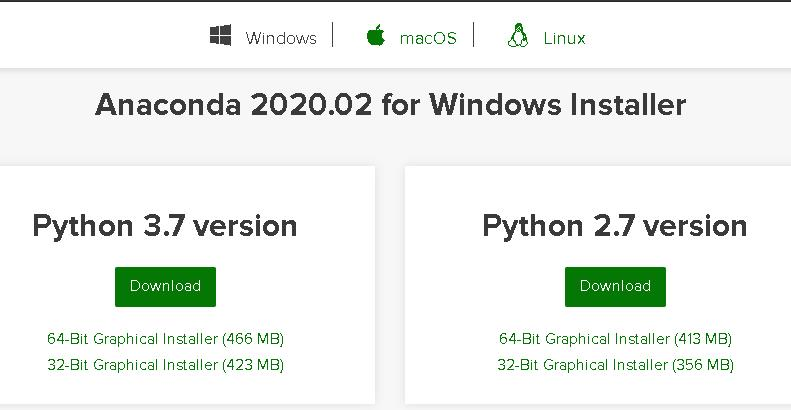
\includegraphics[scale=0.5]{33.1a.jpg}
            \newline
        	b. Mendownload Chromedriver dan meletakkannya di C:/Windows/System32
            \newline
            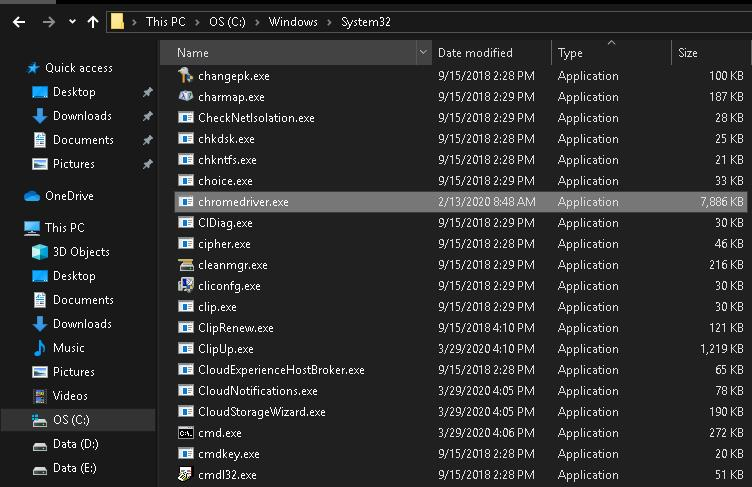
\includegraphics[scale=0.5]{33.1b.jpg}
            \newline
        	c. Menginstall selenium menggunakan cmd (Command Prompt) dengan mengetik “pip install selenium”
            \newline
            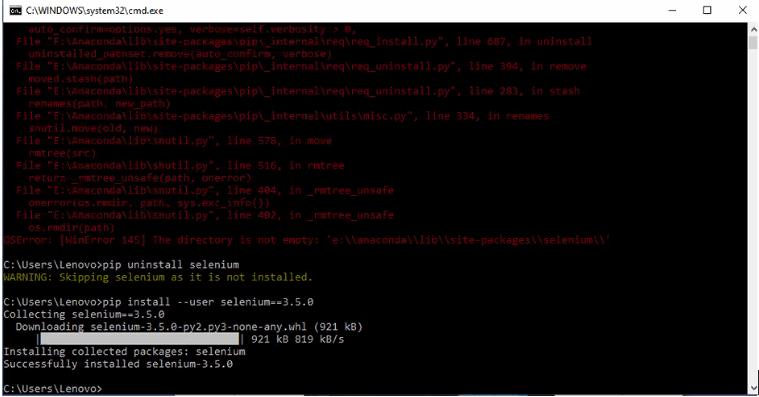
\includegraphics[scale=0.5]{33.1c.jpg}
            \newline
        	d. Membuka Spyder/Visual Studio Code yang sudah terinstall bahasa pemrograman python dan memasukan perintah sebagai berikut
        	\newline
            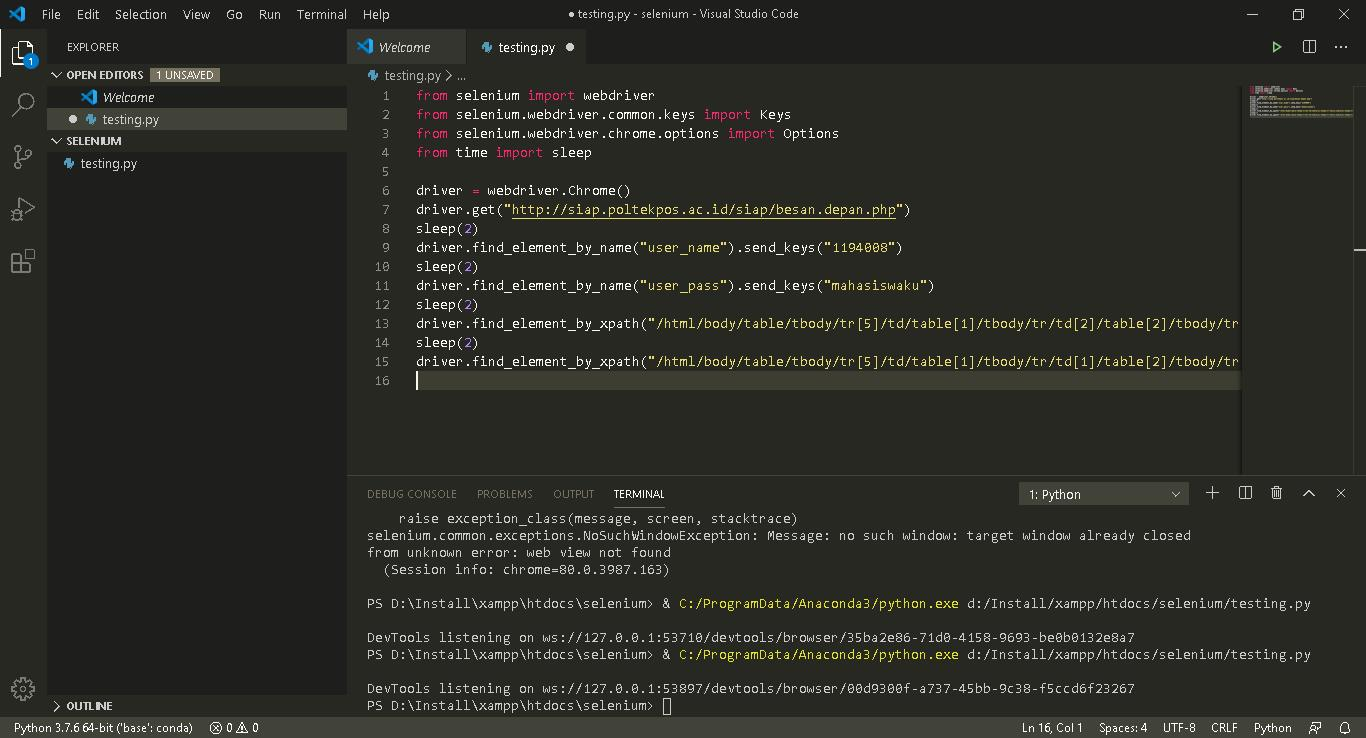
\includegraphics[scale=0.3]{33.1d.jpg}
            \newline
            from selenium import webdriver
            \newline
            from selenium.webdriver.common.keys import Keys
            \newline
            from selenium.webdriver.chrome.options import Options
            \newline
            from time import sleep
            \newline
            \newline
            driver = webdriver.Chrome()
            \newline
            driver.get("http://siap.poltekpos.ac.id/siap/besan.depan.php")
            \newline
            sleep(2)
            \newline
            driver.find\_element\_by\_name("user\_name").send\_keys("1194008")
            \newline
            sleep(2)
            \newline
            driver.find\_element\_by\_name("user\_pass").send\_keys("xxxxxxxxxxx")
            \newline
            sleep(2)
            \newline
            driver.find\_element\_by\_xpath("/html/body/table/tbody/tr[5]/td/table[1]/tbody/tr/td[2]/table[2]/tbody/tr[1]/td[2]/div/form/input[4]").click()
            \newline
            sleep(2)
            \newline
            driver.find\_element\_by\_xpath("/html/body/table/tbody/tr[5]/td/table[1]/tbody/tr/td[1]/table[2]/tbody/tr[1]/td[2]/a[2]").click()
            \newline
            \newline
            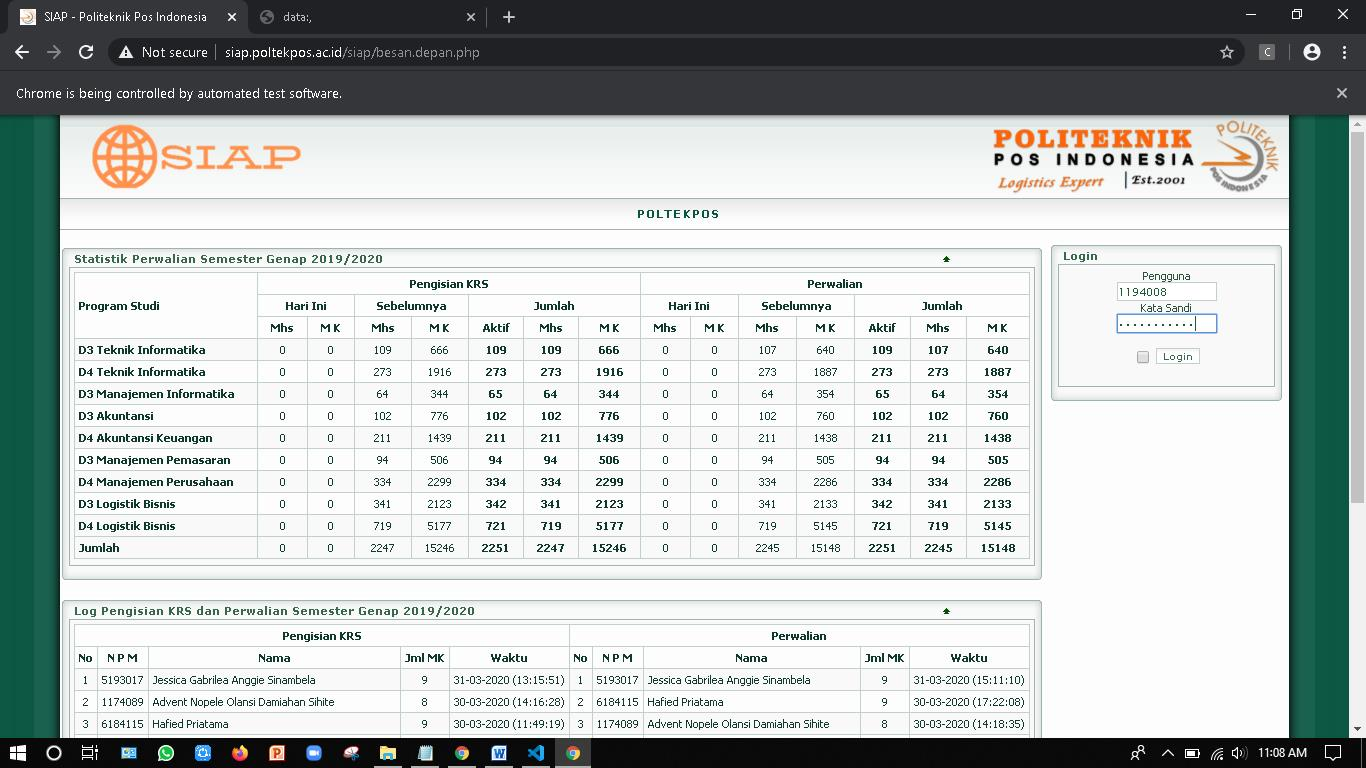
\includegraphics[scale=0.3]{33.1e.jpg}
            \newline
        \item Untuk tugas menginsertkan record masing-masing tabel 34 row kami mengisikan ke 6 table yang tersedia yaitu error\_message, notfound\_message, opening\_message, kelas\_mulai, kelas\_selesai, dan jadwal\_kelas.
            \newline
            \newline
        \item Memasukkan file selenium yang telah dibuat dan laporan pada Github dan mengupdatenya di README.md
           \newline
            	a. Buat folder baru lalu klik kanan pilih “Gitbash Here”	
                \newline
                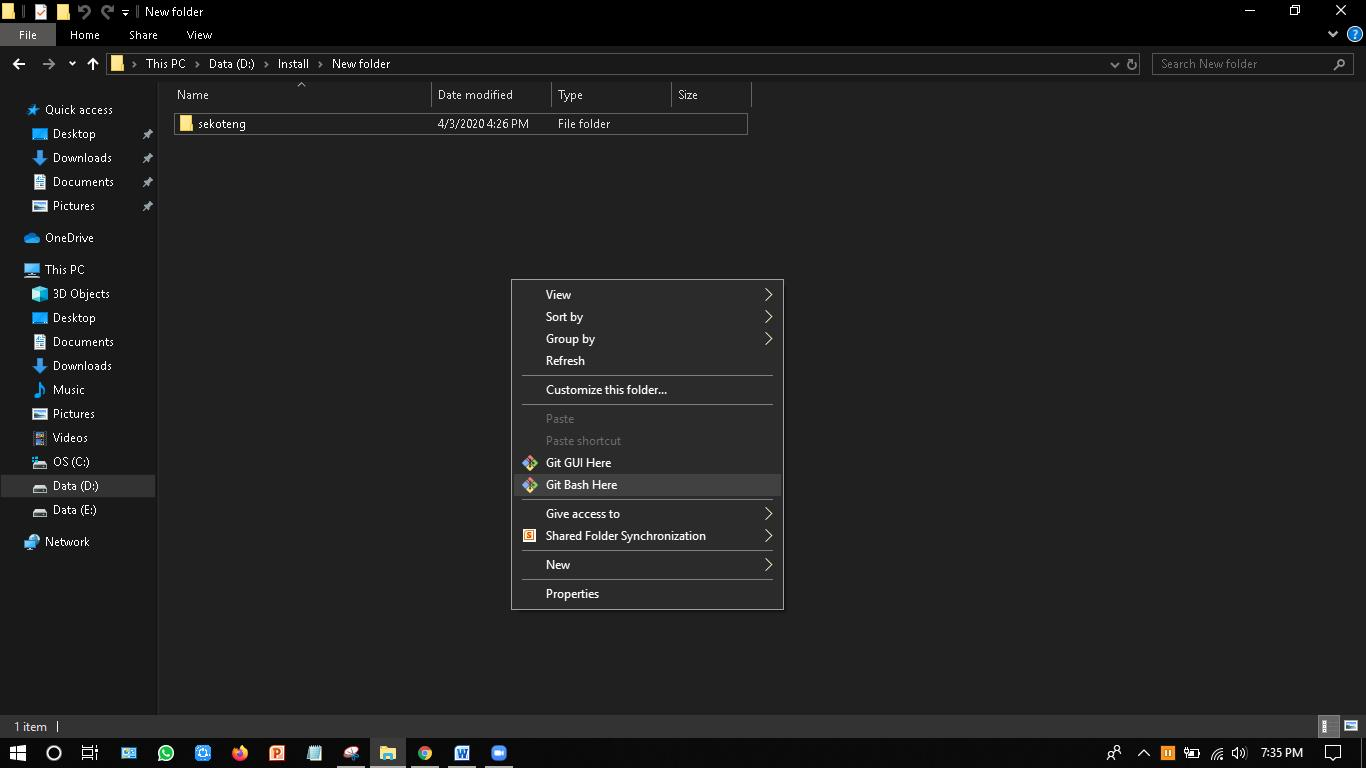
\includegraphics[scale=0.3]{33.3a.jpg}
                \newline
            	b. Buka Github dan pilih repository, lalu clone dan cpy URLnya
                \newline
                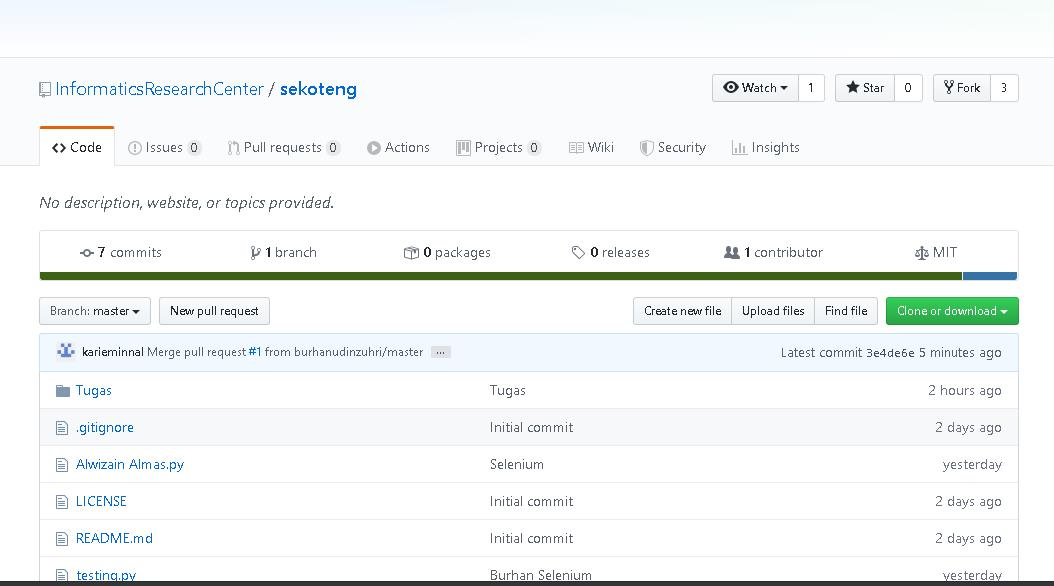
\includegraphics[scale=0.3]{33.3b.jpg}
                \newline
            	c. Masukkan perintah “git clone https://github.com/InformaticsResearchCenter/sekoteng.git”
                \newline
                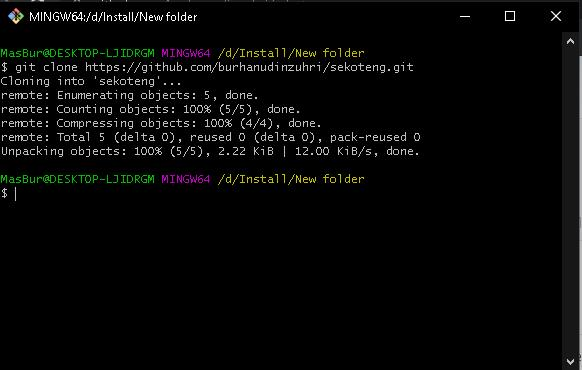
\includegraphics[scale=0.4]{33.3c.jpg}
                \newline
            	d. Setelah selesai maka akan muncul folder baru dengan nama sesui repository, kemudian masukkan file tersebut.
                \newline
                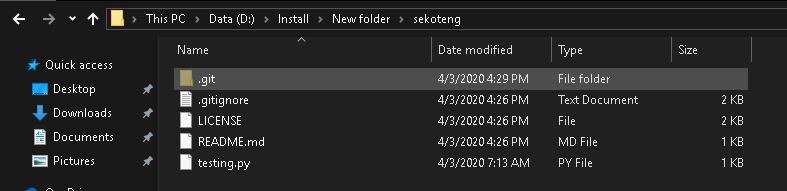
\includegraphics[scale=0.5]{33.3d.jpg}
                \newline
            	e. Klik kanan pada halaman dan pilih Gitbash dan tambahkan perintah seperti dibawah ini
                \newline
                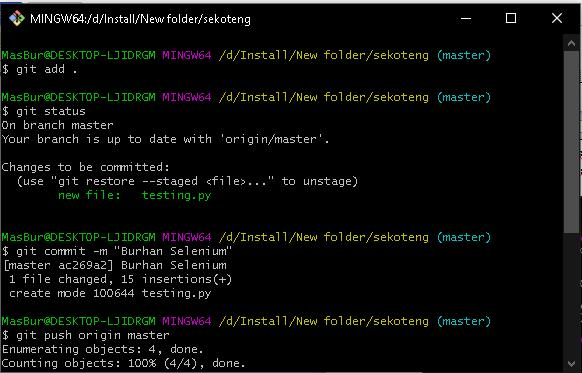
\includegraphics[scale=0.4]{33.3e1.jpg}
                \newline
                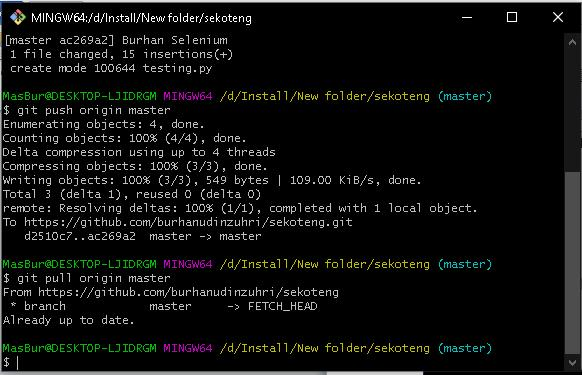
\includegraphics[scale=0.4]{33.3e2.jpg}
                \newline
            	f. Cek kembali file yang tadi diupload dan pull request
                \newline
                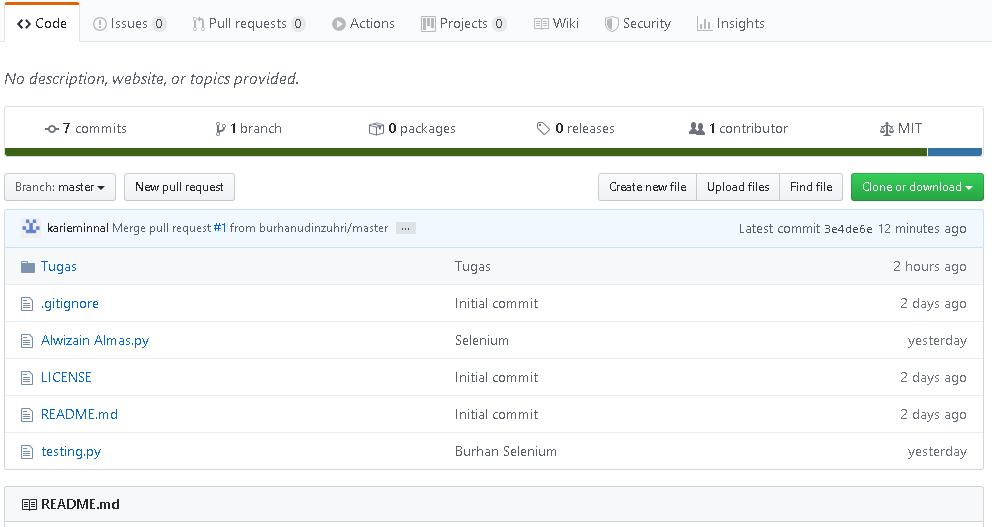
\includegraphics[scale=0.4]{33.3f.jpg}
                \newline
            \seti %harus diketik pada nomor terakhir
        \end{enumerate}
    
\section{Tanggal 3 April 2020:}
Bapak Rolly memberikan perintah kepada saya untuk memperbaiki record yang salah karena terdapat record ganda (double). Serta perintah untuk mengupdate READ.ME yang berada di repository Sekoteng serta menjadwalkan meeting jam 1 siang namun meeting tidak jadi dilaksanakan.
\newline
\newline

\section{Tanggal 5 April 2020:}
Kami menyetorkan alamat Github Sekoteng kepada Bapak Rolly dan menambahkan update lagi pada READ.ME yang berisi jumlah record yang telah kami capai.
\newline
\newline


\section{Tanggal 6 April 2020:}
	Bapak Rolly memberikan 4 tugas yaitu:
		\newline
		\begin{enumerate}
			\item Melakukan perubahan kata SIAP menjadi system akademik pada semua table dengan mengeceknya satu per satu.
			\newline
			\item Mengisi table waiting\_message pada module\_name biodata\_siap\_mahasiswa dan siap\_jadwal masing-masing orang mengisi 20 record.
			\newline
			\item Mengisi table reply pada key\_word panduan masing-masing orang mengisi 10 record.
			\newline
			\item Melakukan Google Meet untuk membahas progres (namun tidak jadi dilaksanakan)
			\newline
			Table waiting\_message pada module\_name biodata\_siap\_mahasiswa
			\newline
			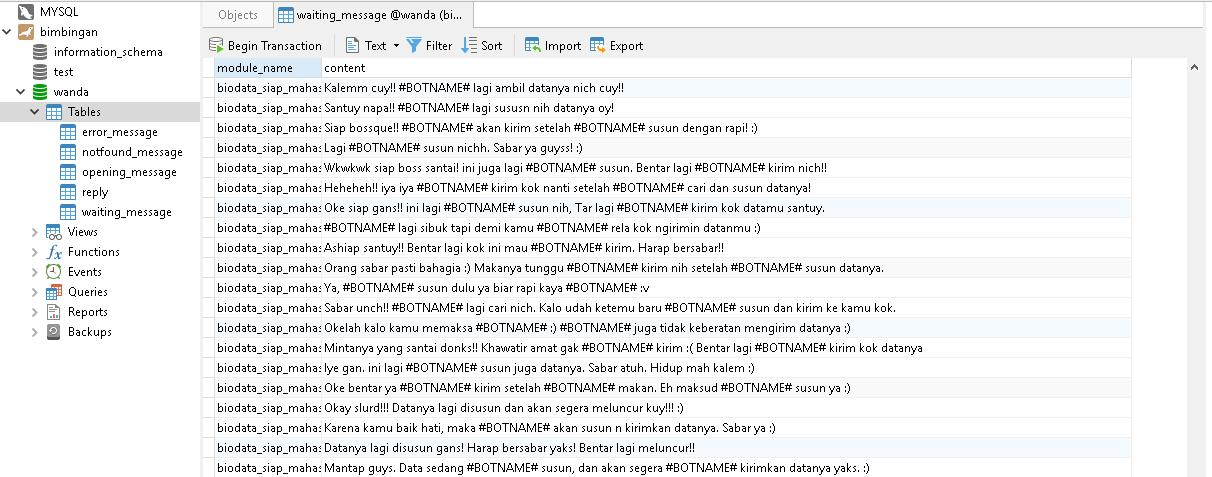
\includegraphics[scale=0.4]{37.1.jpg}
			\newline
			Table waiting\_message pada module\_name biodata\_siap\_mahasiswa siap\_jadwal
			\newline
			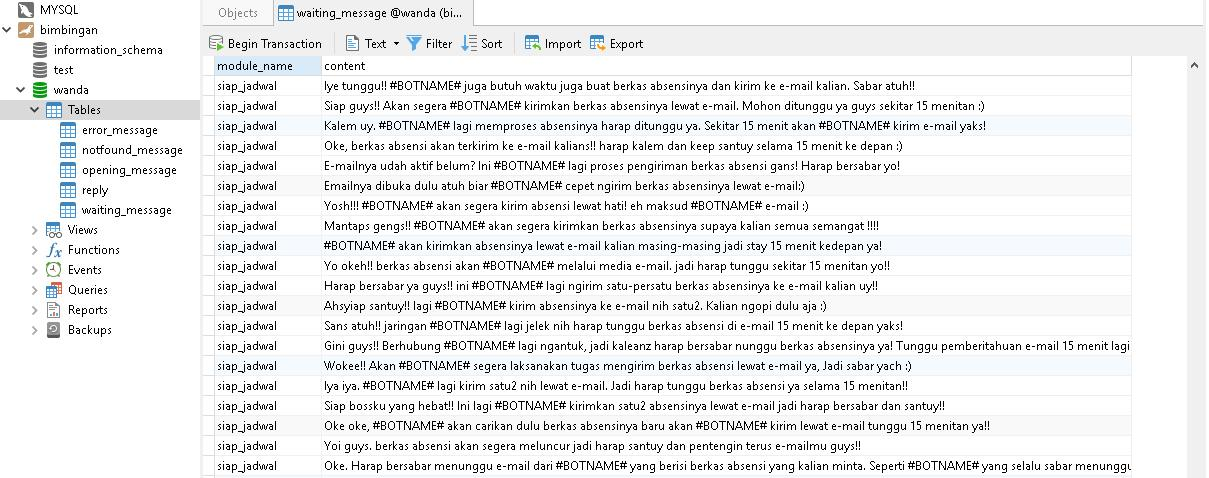
\includegraphics[scale=0.4]{37.2.jpg}
			\newline
			Table reply pada key\_word panduan
			\newline
			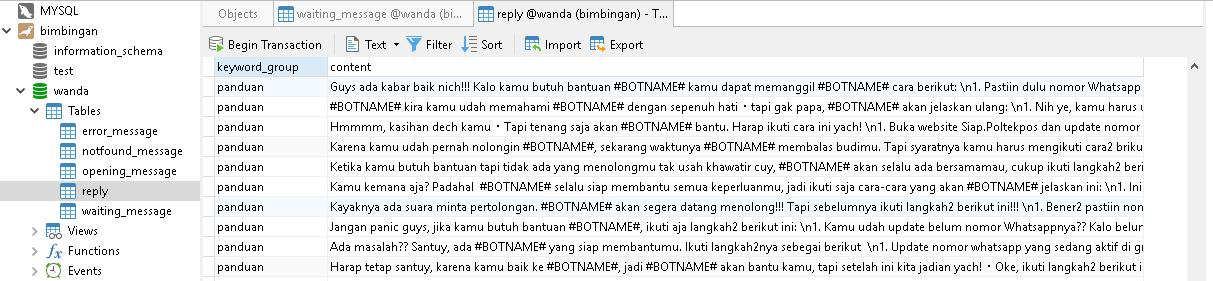
\includegraphics[scale=0.4]{37.3.jpg}
			\newline
			Keterangan table:
			\newline
			a.	 Table biodata\_siap\_mahasiswa
			Merupakan table yang berfungsi sebagai perintah untuk pengguna menunggu biodata mahasiswa dari hasil inputan NPM dan robot akan mengambilkan biodata mahasiswa tersebut. Variable yang terdapat pada table yaitu BOTNAME yang merupakan variable yang berfungsi sebagai nama robot.
			\newline
			b.	Table siap\_jadwal
			Merupakan table yang berfungsi sebagai perintah untuk pengguna menunggu absensi UTS yang akan dikirimkan melalui e-mail masing-masing mahasiswa. Variable yang terdapat pada table yaitu BOTNAME yang merupakan variable yang berfungsi sebagai nama robot.
			\newline
			c.	Table panduan
			Merupakan table yang berisi tata cara menggunakan robot saat mahasiswa membutuhkan bantuan dari robot. Variable yang terdapat pada table yaitu BOTNAME yang merupakan variable yang berfungsi sebagai nama robot.
			\seti %harus diketik pada nomor terakhir
		\end{enumerate}

\section{Tanggal 7 April 2020:}
Bapak Rolly memberi peritah untuk membuka fitur chat dan mengirim pesan menggunakan selenium. Untuk kelompok Sekoteng mendapatkan bagian Veronika yang merupakan chatbot dari Telkomsel. Serta perintah untuk mengisi table reply pada key\_word buli, trims, pujian, dan joke masing-masing orang mengisi 10 record.
	\newline 
	\begin{enumerate}
		\item Mengirim pesan menggunakan selenium
			\newline
			a. Berikut merupakan codingan yang saya gunakan:
			\newline
			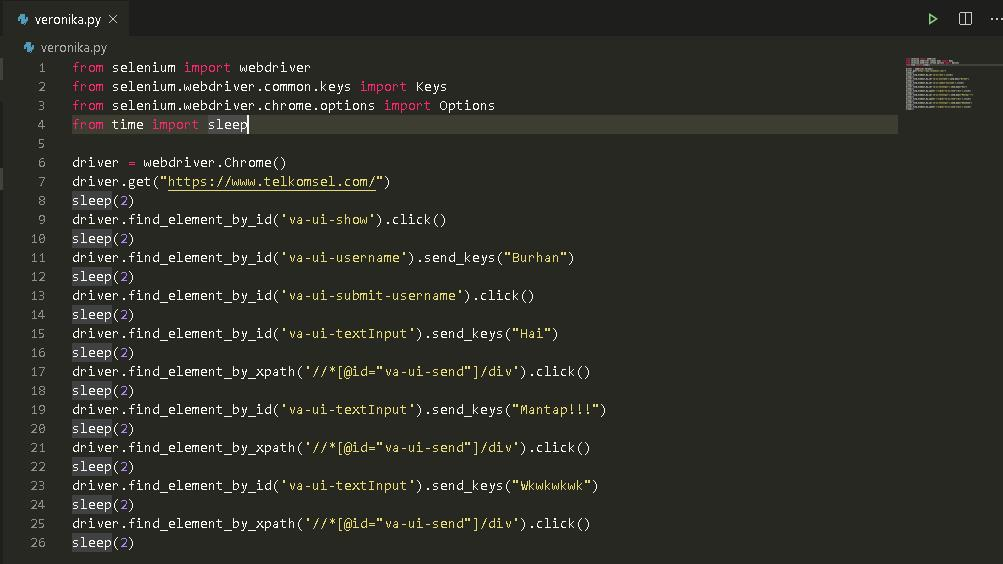
\includegraphics[scale=0.4]{38.1a.jpg}
			\newline
			from selenium import webdriver
			from selenium.webdriver.common.keys import Keys
			from selenium.webdriver.chrome.options import Options
			from time import sleep
			\newline
			driver = webdriver.Chrome()
			driver.get("https://www.telkomsel.com/")
			sleep(2)
			driver.find\_element\_by\_id('va-ui-show').click()
			sleep(2)
			driver.find\_element\_by\_id('va-ui-username').send\_keys("Burhan")
			sleep(2)
			driver.find\_element\_by\_id('va-ui-submit-username').click()
			sleep(2)
			driver.find\_element\_by\_id('va-ui-textInput').send\_keys("Hai")
			sleep(2)
			driver.find\_element\_by\_xpath('//*[@id="va-ui-send"]/div').click()
			sleep(2)
			driver.find\_element\_by\_id('va-ui-textInput').send\_keys("Mantap!!!")
			sleep(2)
			driver.find\_element\_by\_xpath('//*[@id="va-ui-send"]/div').click()
			sleep(2)
			driver.find\_element\_by\_id('va-ui-textInput').send\_keys("Wkwkwkwk")
			sleep(2)
			driver.find\_element\_by\_xpath('//*[@id="va-ui-send"]/div').click()
			sleep(2)
			\newline
			b. Berikut merupakan hasilnya:
			\newline
			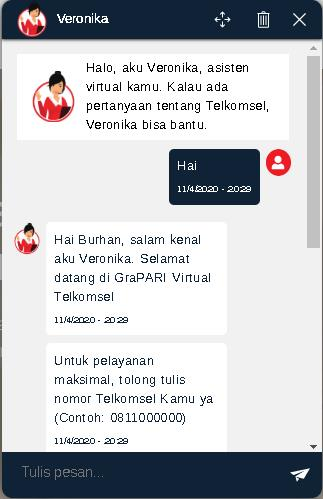
\includegraphics[scale=0.4]{38.1b.jpg}
			\newline
		\item Mengisis record table reply pada key\_word buli, trims, pujian, dan joke
		\newline
		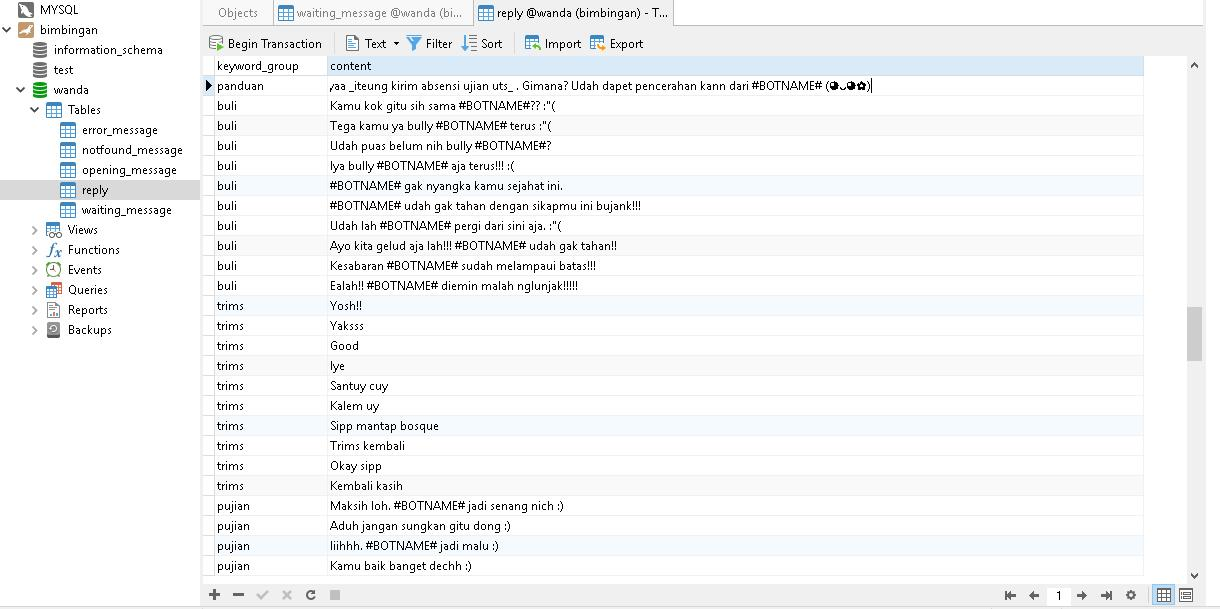
\includegraphics[scale=0.4]{38.2.jpg}
		\newline
		Keterangan table:
		\newline
		a.	Table reply pada key\_word buli
		Merupakan table yang berfungsi sebagai pesan untuk pengguna yang berisi respon robot ketika dibuli pengguna. Variable yang terdapat pada table yaitu BOTNAME yang merupakan variable yang berfungsi sebagai nama robot.
		\newline
		b.	Table reply pada key\_word trims
		Merupakan table yang berfungsi sebagai pesan untuk pengguna yang berisi respon robot ketika pengguna mengucapkan terima kasih kepada robot. Variable yang terdapat pada table yaitu BOTNAME yang merupakan variable yang berfungsi sebagai nama robot.
		\newline
		c.	Table reply pada key\_word pujian
		Merupakan table yang berfungsi sebagai pesan untuk pengguna yang berisi respon robot ketika dipuji pengguna. Variable yang terdapat pada table yaitu BOTNAME yang merupakan variable yang berfungsi sebagai nama robot.
		\newline
		d.	Table reply pada key\_word joke
		Merupakan table yang berfungsi sebagai pesan untuk pengguna yang berisi respon robot ketika pengguna meminta robot untuk memberikan lelucon. Variable yang terdapat pada table yaitu BOTNAME yang merupakan variable yang berfungsi sebagai nama robot.
		\newline
		\newline
		\seti %harus diketik pada nomor terakhir
	\end{enumerate}


\section{Tanggal 8 April 2020:}
Bapak Rolly memberikan perintah untuk mengupdate READ.ME yang ada di Github dan memperbaiki bahasa pada chatbot yang kiranya masih kasar dan kurang cocok jika dipakai oleh seluruh jajaran POLTEKPOS.
\newline
\newline

\section{Tanggal 9 April 2020:}
Bapak Rolly memberikan 4 tugas yaitu:
	\newline
	\begin{enumerate}
			\item Melakukan meeting dan membahas tentang progres selenium.
			\newline
			\item Membuat video tutorial menggunakan selenium untuk membuka chat dan mengirim pesan serta menguploadnya di YouTube. Ketentuan videonya yaitu harus menggunakan intro yang sudah Bapak tentukan.
			\newline
			\item Membuat chatbot pada Telegram yang memiliki deadline Senin tanggal 12 April 2020.
			\newline
			\item Mengganti respon pada chatbot untuk jadwal menjadi absensi.
			\newline
		\seti %harus diketik pada nomor terakhir
	\end{enumerate}

\section{Tanggal 10 April 2020:}
Kami telah menyelesaikan tugas untuk mengganti kata “jadwal” menjadi kata “absensi” pada table waiting\_message module\_name siap\_jadwal.
	\newline
	\newline

\section{Tanggal 13 April 2020:}
Kami telah menyelesaikan tugas membuat chatbot di Telegram sesuai deadline yang ditentukan.
	\newline
	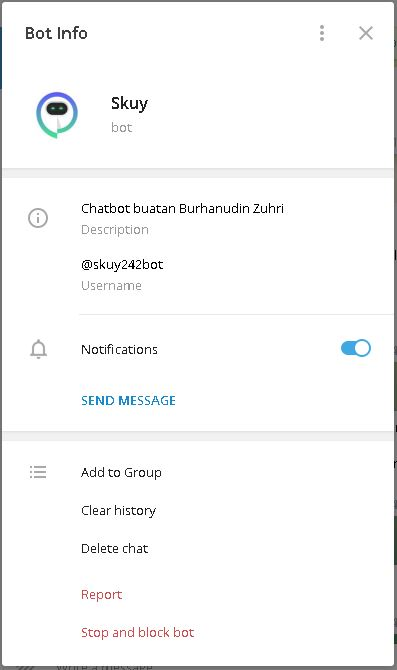
\includegraphics[scale=0.5]{0.jpg}
	\newline

\section{Tanggal 14 April 2020:}
Bapak Rolly memberikan tugas untuk menghubungkan Veronika dengan Bot di Telegram sehingga pesan dari Telegram dapat diteruskan ke Veronika.
	\newline
	\newline

\section{Tanggal 18 April 2020:}
Kak Tri Angga Dio S. memberikan tugas untuk mengisi record iteung untuk module siap\_jadwal serta manambahkan variable EMAIL sebanyak 20 record masing-masing orang.
	\newline
	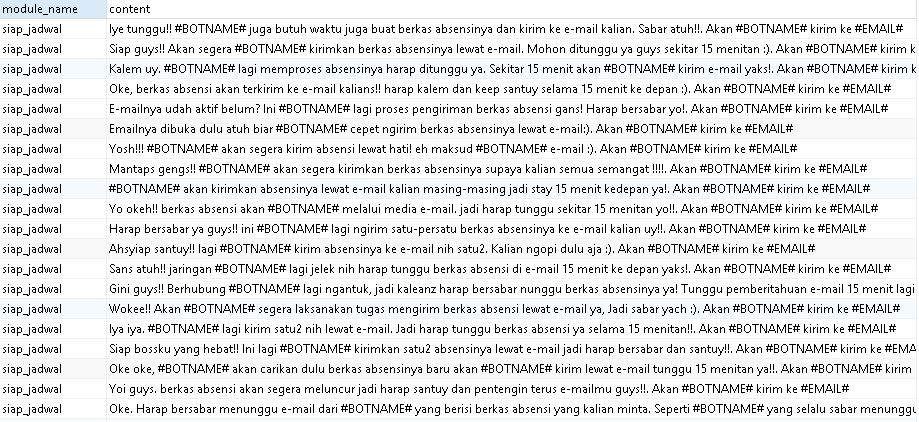
\includegraphics[scale=0.5]{1.jpg}
	\newline

\section{Tanggal 20 April 2020:}
Bapak Rolly memberikan saran untuk melakukan meeting dengan Kak Wahyu dan Kak Innal untuk menyelesaikan masalah penghubungan Veronika dengan Bot di Telegram. Serta membuat laporannya dan buku panduan tata cara penggunaan secara detail untuk pemula sesegera mungkin.
	\newline
	\newline

\section{Tanggal 22 April 2020:}
Bapak Rolly memberikan tugas untuk menginputkan record pada table waiting\_message module\_name jadwal\_ujian sebanyak 20 record per orang.
	\newline
	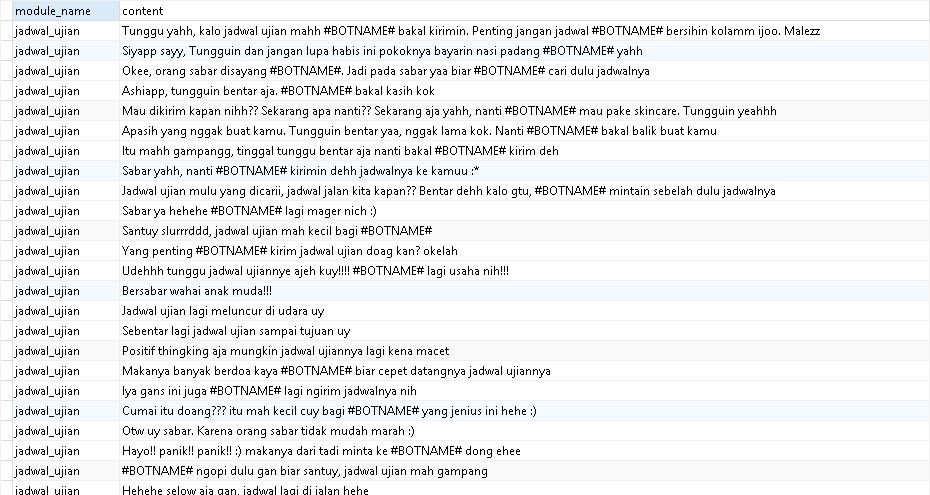
\includegraphics[scale=0.5]{2.jpg}
	\newline

\section{Tanggal 24 April 2020:}
Bapak Rolly memberikan tugas untuk memperbaiki record error\_message yang salah input ke notfound\_message.
	\newline
	\newline

\section{Tanggal 29 April 2020:}
Kami mengirim Deskripsi Aplikasi pada bimbingan simpro dan diterima oleh Bapak Rolly.
	\newline
	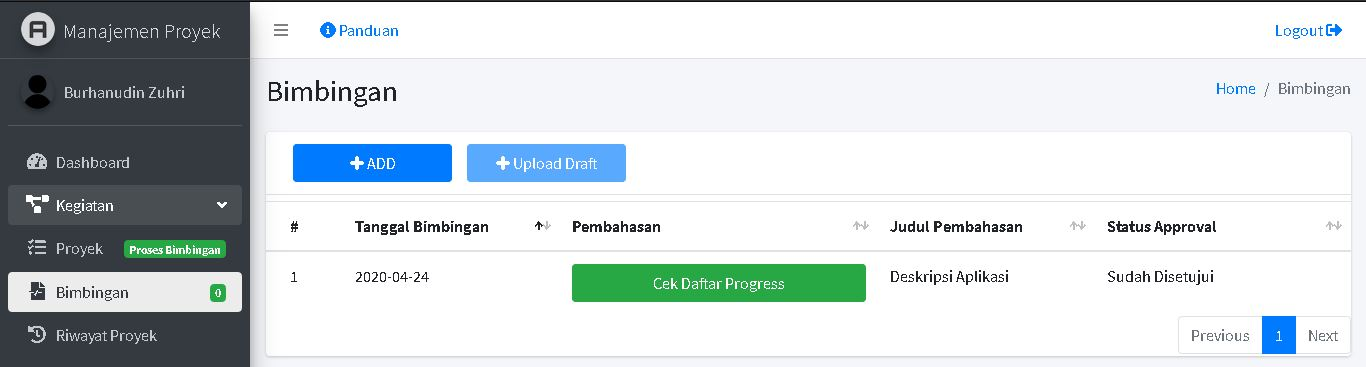
\includegraphics[scale=0.3]{3a.jpg}
	\newline
	\newline
	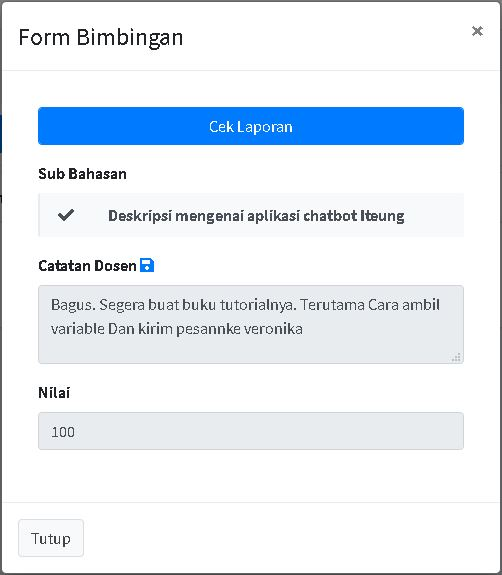
\includegraphics[scale=0.5]{3b.jpg}
	\newline

\section{Tanggal 4 Mei 2020:}
Bapak Rolly menyarankan untuk menonton siding kakak tingkat tentang proyek yang dikerjakannya.
	\newline
	\newline
	
\section{Tanggal 5 Mei 2020:}
Bapak Rolly memberikan tugas untuk mengupdate panduan iteung sehingga dapat menyesuaikan dengan fitur yang terbaru.
	\newline
	\includegraphics[scale=0.5]{4.jpg}
	\newline

\section{Tanggal 6 Mei 2020:}
Kami merevisi pekerjaan kami tentang panduan iteung.
	\newline
	\newline

\section{Tanggal 12 Mei 2020:}
Kami menanyakan cara membaca dan mengambil variable sms melalui hp dan Bapak Rolly menyuruh kami untuk melakukan google meet dengan Kak Innal, Kak Wahyu, dan Kak Kadek.
	\newline
	\newline

\section{Tanggal 13 Mei 2020:}
Kami telah menyelesaikan menghubungkan Veronika dengan Bot di Telegram dan bapak Rolly meminta kami untuk membuat laporan dan demo di youtube serta melakukan sidang. 
	\newline
	\newline
	
\section{Tanggal 14 Mei 2020:}
Kami menayakan tentang cara menampilkan balasan veronica di Telegram dengan cara melakukan copy full xpath dan menambahkan .text di belakang codenya.
Membuat video demo di youtube masing-masing individu
	\newline
	\newline


\section{Tanggal 21 Mei 2020:}
Kami mengirim link video demo selenium di youtube. Berikut link videonya :
https://youtu.be/\_0nnIstisYE
	\newline
	Bapak memberi tugas :
	\begin{enumerate}
		\item Mode headless
		\newline
		\item Perintah langsung cek kuota 
		\newline
		\seti %harus diketik pada nomor terakhir
	\end{enumerate}
	
\section{Tanggal 22 Juni 2020:}
Bapak Rolly memberi tugas untuk share informasi tentang seminar Informatic Webinar Series.
	\newline
	\newline


	

\end{document}